\documentclass[tikz]{standalone}

\usetikzlibrary{intersections}

\begin{document}
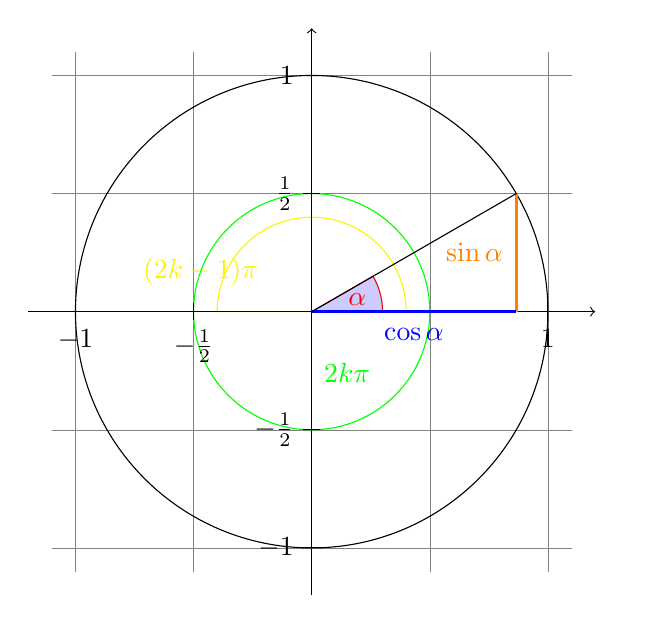
\begin{tikzpicture}[scale=3]
    \draw[step=.5cm,gray,very thin] (-1.1,-1.1) grid (1.1,1.1);
    \filldraw[fill=blue!20,draw=red] (0,0) -- (3mm,0mm)
    arc [start angle=0, end angle=30, radius=3mm] -- cycle;
    \node[red] at (15:2mm) {$\alpha$};
    \filldraw[fill=none,draw=yellow] (0,0) -- (4mm,0mm)
    arc [start angle=0, end angle=180, radius=4mm] -- cycle;
    \node[yellow] at (160:5mm) {$(2k-1)\pi$};
    \filldraw[fill=none,draw=green] (0,0) -- (5mm,0mm)
    arc [start angle=0, end angle=360, radius=5mm] -- cycle;
    \node[green] at (-60:3mm) {$2k\pi$};
    \draw[->] (-1.2,0) -- (1.2,0) coordinate (x axis);
    \draw[->] (0,-1.2) -- (0,1.2) coordinate (y axis);
    \draw (0,0) circle [radius=1cm];
    \draw[very thick,orange]
    (30:1cm) -- node[left=1pt] {$\sin \alpha$} (30:1cm |- x axis);
    \draw[very thick,blue]
    (30:1cm |- x axis) -- node[below=2pt] {$\cos \alpha$} (0,0);
    \path [name path=upward line] (1,0) -- (1,1);
    \path [name path=sloped line] (0,0) -- (30:1.5cm);
    \draw (0,0) -- (30:1cm);
    \foreach \x/\xtext in {-1, -0.5/-\frac{1}{2}, 1}
    \draw (\x cm,1pt) -- (\x cm,-1pt) node[anchor=north] {$\xtext$};
    \foreach \y/\ytext in {-1, -0.5/-\frac{1}{2}, 0.5/\frac{1}{2}, 1}
    \draw (1pt,\y cm) -- (-1pt,\y cm) node[anchor=east] {$\ytext$};
\end{tikzpicture}
\end{document}
